\chapter{Layered Architecture}


\section{Introduction}

The layered architecture style, often referred to as n-tier architecture, is commonly used for developing a wide range of applications. It is particularly favored because of its straightforward approach, which mirrors the division of labor found in many development organizations. For example, in a typical enterprise, different teams may handle the UI, backend, business logic, and database management. This separation of concerns naturally maps onto the layers of a typical layered architecture. The style is often chosen by default, especially when teams are uncertain about which architecture to use, as it provides a well-defined, modular structure.

One of the key advantages of layered architecture is its ability to isolate different technical aspects of the application into logical layers. These layers typically include presentation, business, persistence, and database layers, each responsible for specific tasks. This isolation makes it easier to assign roles and responsibilities, allowing developers to focus on their expertise. However, as applications grow larger and more complex, the drawbacks of this approach, such as reduced flexibility and increased difficulty in adapting to change, become more evident. In such cases, it may be necessary to explore other architecture styles that offer more modularity and scalability.

\section{Background}

The layered architecture exists as a solution to the increasing complexity of software systems. Over time, developers and architects realized that as systems grew larger, it became increasingly difficult to manage and maintain them without a clear structure. Software systems, especially enterprise applications, often consist of various components such as user interfaces, business logic, and data storage. The layered architecture was introduced to address this complexity by organizing these components into distinct layers, each with its own responsibility. This separation simplifies the development process, enhances maintainability, and allows teams to focus on specific areas of functionality without the need to understand the entire system.

The core idea behind the layered architecture is to provide a clear separation of concerns. By breaking down an application into layers, it becomes easier to manage, update, and scale the system over time. For example, changes to the user interface (UI) layer can be made independently of changes to the business logic or the database layer. This modular approach allows teams to work in parallel on different parts of the system, improving efficiency and reducing the risk of introducing errors.

Moreover, the layered architecture style promotes reuse and standardization. By defining standard interfaces between layers, different developers or teams can work on different layers without stepping on each other’s toes. For instance, a UI developer can focus on how data is presented to the user, while a backend developer can focus on handling business rules and interacting with the database, without needing to worry about the other layer's implementation details.

The layered architecture also aids in testing and debugging. Since each layer has a distinct responsibility, it becomes easier to isolate and identify issues. Developers can test individual layers in isolation before integrating them into the full system, making it easier to find bugs and maintain system integrity.

In summary, the layered architecture exists as a solution to the growing need for structure and organization in software development. It provides a clear separation of concerns, supports modular development, enhances maintainability, and promotes better testing practices, all of which help developers manage the complexity of modern applications.

\section{History}

The layered architecture style has its roots in the early days of software engineering and is closely associated with the development of large-scale, enterprise-level applications. The concept of separating functionality into distinct layers was not introduced by a single individual but emerged gradually over time as software systems grew in complexity and scale. 

\begin{enumerate}
	\item \textbf{Early Software Design}: 
	In the 1960s and 1970s, software systems were often monolithic, with little to no separation between the user interface, business logic, and data storage components. As applications grew in size, the lack of structure became problematic, leading to difficulties in maintaining and updating these systems. Developers began to recognize the need for modularization and abstraction, which laid the foundation for layered designs.
	
	\item \textbf{The Birth of Layered Concepts}: 
	In the 1980s, as object-oriented programming (OOP) became more widely adopted, the idea of organizing software components into layers started to take shape. The layered architecture as we know it today was formalized during this period, driven by the need to separate concerns and create more maintainable and scalable systems. Layered architecture became popular in both academic circles and real-world software development as a way to deal with growing complexity.
	
	\item \textbf{The Rise of Client-Server Architectures}: 
	During the 1990s, the client-server model gained widespread adoption, and layered architecture began to be used in the context of distributed systems. Client applications were often designed to handle the presentation layer, while the server handled business logic and data persistence. This era saw the establishment of the "four-tier architecture" (presentation, business, persistence, and database), which became a standard template for enterprise applications.
	
	\item \textbf{The 2000s and Web Development}: 
	The 2000s saw the rise of web applications, which further popularized the layered architecture. The Model-View-Controller (MVC) pattern, often associated with web frameworks like Ruby on Rails and Spring, is a direct evolution of the layered architecture. The MVC pattern emphasizes the separation of concerns between data (Model), presentation (View), and user interaction (Controller), mirroring the original principles of layered architecture.
	
	\item \textbf{Contemporary Use}: 
	In the 2010s and beyond, layered architecture remained a standard approach for many enterprise systems. Despite the rise of microservices and more modular architectures, layered architecture continues to be relevant, particularly in small to medium-sized applications, monolithic systems, and web development. Its simplicity and clear structure continue to make it an appealing choice for many developers, especially when time or budget constraints are a factor.
	
	\item \textbf{Layered Architecture and Microservices}: 
	With the rise of microservices architectures in recent years, the concept of layering has been adapted. While microservices break down applications into independent services, the underlying principle of separating concerns into logical layers remains important. Even in microservices, there are often layers for presentation, business logic, and data persistence, though these layers may exist within individual microservices rather than a single monolithic application.
\end{enumerate}

In conclusion, the history of layered architecture is marked by its evolution from early monolithic designs to modern, distributed systems. Its foundational principles of separation of concerns, modularity, and maintainability continue to be central to its widespread use in both traditional and modern software development contexts.


\section{Layered Architecture Topology}

\begin{figure}[ht]
	\centering
	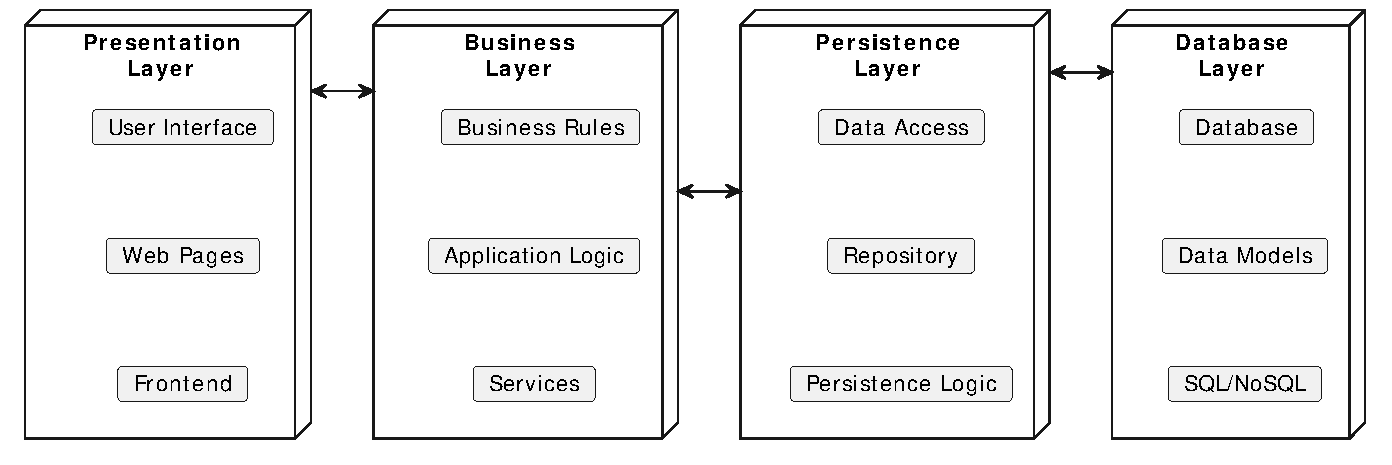
\includegraphics[width=\textwidth]{../images/out/layered_architecture.pdf}
	\caption{Layered Architecture Diagram}
	\label{fig:layered_architecture}
\end{figure}

The architecture presented here follows a layered structure, often referred to as a \textbf{four-layered architecture}, which helps in organizing and structuring software applications in a way that separates concerns and improves maintainability, scalability, and flexibility. In this section, we will discuss the layers in detail, examining their roles and responsibilities, as well as how they interact with one another. One instance of layered architecture is a topology that consists of presentation, business, persistence, and database layers. Of course, there are other instances of layered architecture, such as Containerized Architecture (App Layer, Docker Layer, Host OS Layer, Infrastructure Layer), OSI Model (Application Layer, Presentation Layer, Session Layer, Microkernel Architecture (Core Layer, Extension Layer), etc.

\subsection{Presentation Layer}

The \textbf{Presentation Layer} is the topmost layer of the architecture, designed to manage the interaction between the user and the system. It is responsible for presenting information to the user and receiving input from the user. In the context of web applications, this layer typically includes elements like web pages, user interfaces, and the frontend logic. Components in this layer handle user requests and present the data in a user-friendly format.

In the diagram, this layer consists of the following components:
\begin{itemize}
	\item \textbf{User Interface (UI)}: The part of the application that the user interacts with directly, including buttons, forms, and other interface elements.
	\item \textbf{Web Pages}: The various pages that make up the application’s frontend, such as home pages, dashboards, and form submissions.
	\item \textbf{Frontend}: The overall frontend architecture, which might include JavaScript, CSS, and HTML, as well as frameworks like React or Angular.
\end{itemize}

The Presentation Layer communicates with the next layer, the Business Layer, to fetch or send data based on user interactions.

\subsection{Business Layer}

The \textbf{Business Layer}, also known as the \textit{Application Logic} or \textit{Domain Logic} layer, is where the core functionality of the application resides. This layer is responsible for implementing business rules and logic that define how the application should behave. It encapsulates the decisions, processes, and actions that drive the application’s functionality. 

In the diagram, this layer includes, but not limited to, the following components:
\begin{itemize}
	\item \textbf{Business Rules}: These define the core principles and rules of the system, such as how calculations are performed or how data is validated.
	\item \textbf{Application Logic}: This refers to the detailed rules and processes that make up the application’s operation, including handling user input and managing state transitions.
	\item \textbf{Services}: Services may include external services or internal service layers that perform specific tasks, such as sending emails, processing payments, or managing sessions.
\end{itemize}

The Business Layer acts as a mediator between the Presentation and Persistence layers. It is in this layer where business logic is applied, and it decides which data to retrieve or modify from the Persistence Layer based on user actions in the Presentation Layer.

\subsection{Persistence Layer}

The \textbf{Persistence Layer} is responsible for managing the data access and storage of the application. It defines how data is stored, retrieved, and updated, typically using databases or other forms of storage. This layer ensures that the business logic can interact with data without directly dealing with low-level storage operations.

In the diagram, the Persistence Layer consists of, but not limited to, the following components:
\begin{itemize}
	\item \textbf{Data Access}: This component handles the interaction with data storage systems, providing the necessary queries or commands to interact with the database.
	\item \textbf{Repository}: A repository serves as a collection of objects that abstract the retrieval, update, and deletion of data entities.
	\item \textbf{Persistence Logic}: The logic that governs how data is stored, ensuring that the data is in a consistent and retrievable state.
\end{itemize}

This layer communicates with the Database Layer, ensuring that data is accurately and efficiently stored and retrieved when needed by the Business Layer.

\subsection{Database Layer}

The \textbf{Database Layer} is the foundational layer where data is stored persistently. It includes the database itself and the data models that represent the structure of the data. This layer is responsible for ensuring the integrity, consistency, and security of the data.

In the diagram, this layer consists of, but not limited to, the following components:
\begin{itemize}
	\item \textbf{Database}: The actual database system used to store application data, such as MySQL, PostgreSQL, or NoSQL databases like MongoDB.
	\item \textbf{Data Models}: The data models define the structure of the data stored in the database, such as tables in relational databases or collections in NoSQL systems.
	\item \textbf{SQL/NoSQL}: Refers to the types of databases used, whether structured query language (SQL) databases like MySQL or non-relational (NoSQL) databases like MongoDB, each having its own specific use cases.
\end{itemize}

The Database Layer provides data persistence and integrity, ensuring that data remains available even after the application has been shut down or restarted.

\subsection{Layer Interactions}

Each of these layers communicates with adjacent layers to fulfill the application’s requirements. The flow of data can be described as follows:

\begin{itemize}
	\item The \textbf{Presentation Layer} sends user input to the \textbf{Business Layer}, requesting operations or data retrieval.
	\item The \textbf{Business Layer} processes the request, applying business logic, and then communicates with the \textbf{Persistence Layer} to retrieve or modify data.
	\item The \textbf{Persistence Layer} accesses the database, performing the necessary operations to satisfy the request from the Business Layer.
	\item The \textbf{Database Layer} provides the data to the Persistence Layer, which then sends it back to the Business Layer, and eventually the Presentation Layer, where it is presented to the user.
\end{itemize}

By using a layered architecture, the system maintains a high degree of separation of concerns, ensuring that each layer is responsible for a specific aspect of the application’s operation. This separation makes it easier to modify, extend, or replace individual components without affecting the rest of the system.

\section{Closed and Open Layer Architectures}

In software design, layered architecture plays a pivotal role in organizing the system's components. A common pattern involves the use of closed and open layers, which determine the degree of interaction and accessibility between various system components. The diagram below illustrates the concepts of closed and open layers in a system architecture.

\begin{figure}[ht]
	\centering
	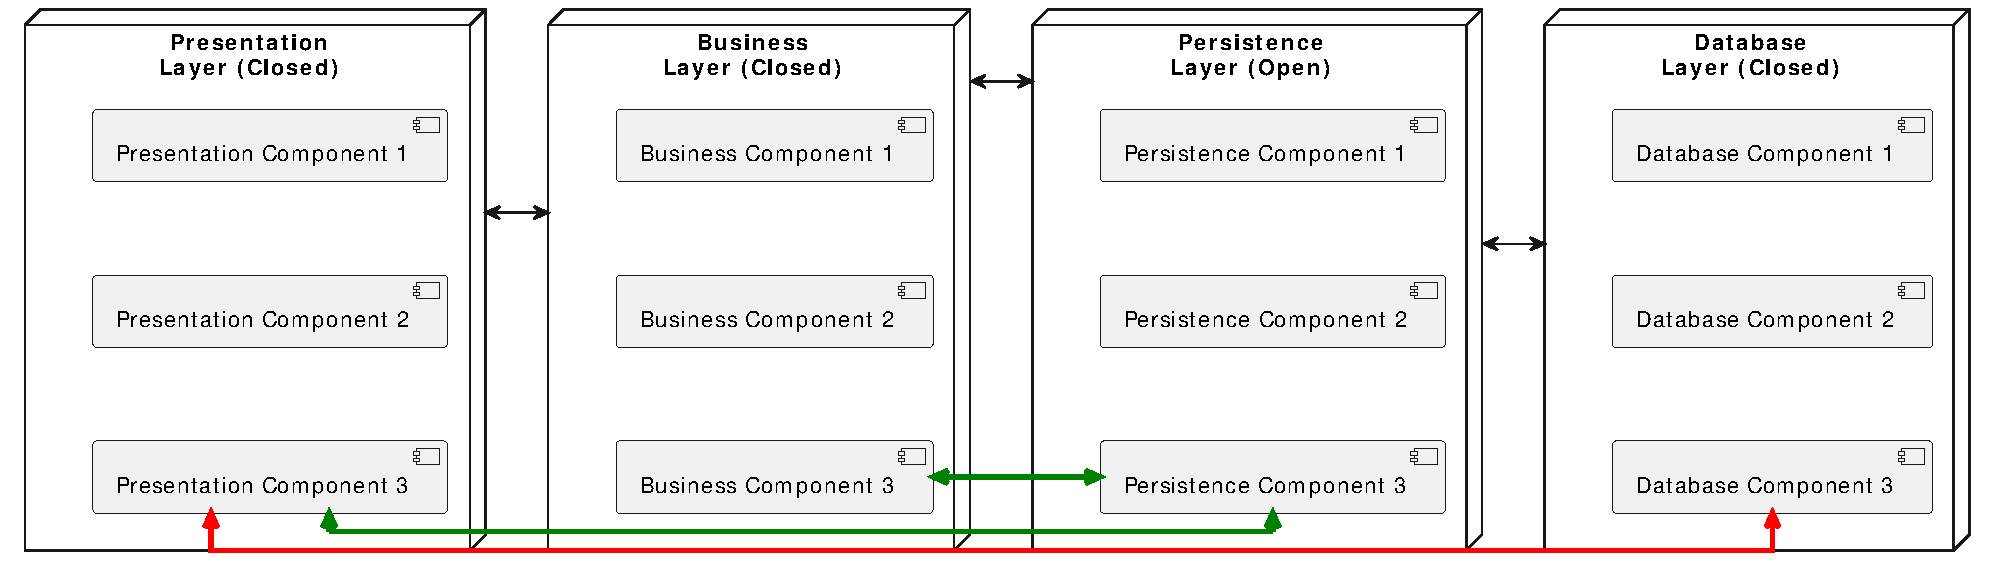
\includegraphics[width=\textwidth]{../images/out/layered_architecture_open.pdf}
	\caption{Closed and Open Layer Architectures}
	\label{fig:layered_architecture_open}
\end{figure}

\subsection{Closed Layer Architecture}

A closed layer architecture refers to layers where components within the layer can only interact with other components within the same layer or with adjacent layers. This restricts direct external access to the components of the layer. The closed nature of these layers provides security, stability, and encapsulation of logic. 

In the diagram, both the \textbf{Presentation Layer} and the \textbf{Database Layer} are considered closed layers. The components within these layers are isolated from external interactions. Specifically:
\begin{enumerate}
	\item The \textbf{Presentation Layer} consists of components such as \textit{Presentation Component 1}, \textit{Presentation Component 2}, and \textit{Presentation Component 3}. These components interact only with adjacent layers and not with external entities directly.
	\item The \textbf{Database Layer} comprises components like \textit{Database Component 1}, \textit{Database Component 2}, and \textit{Database Component 3}. These components are shielded from direct external modifications.
\end{enumerate}

It is important to note that the red connection between \textit{Presentation Component 3} and \textit{Database Component 3} is prohibited because the \textbf{Database Layer} is closed. In a closed layer architecture, components within the layer should not have direct access to or interact with external layers outside of the adjacent layer. Therefore, any communication between the \textbf{Presentation Layer} and the \textbf{Database Layer} must occur through the \textbf{Persistence Layer}, which acts as the intermediary.

This prohibition ensures that the closed nature of the layers is maintained, enforcing proper encapsulation, and keeping the system's components well-separated. The access from \textit{Presentation Component 3} to \textit{Database Component 3} would break this rule and is therefore not allowed in this architecture.

Examples where a closed layer architecture is preferred include:
\begin{enumerate}
	\item \textbf{Banking Systems:} In banking applications, the \textbf{Presentation Layer} (e.g., web interfaces, mobile apps) and the \textbf{Database Layer} (e.g., user data, transaction records) must remain isolated to ensure sensitive data is not exposed. This design prevents any direct interaction between the user interface and the database, mitigating the risk of data breaches.
	\item \textbf{Healthcare Systems:} In healthcare applications, patient data and treatment records stored in the \textbf{Database Layer} should not be directly accessible by the \textbf{Presentation Layer}. Instead, any access to the database should go through the \textbf{Persistence Layer} to ensure data validation, security, and privacy regulations are enforced.
\end{enumerate}

\subsection{Open Layer Architecture}

An open layer allows greater flexibility and external interaction. Open layers expose their components to communication from other layers, making them more adaptable for various integrations. The open nature of these layers enables data exchange and functionality access across layers.

In the provided diagram, the \textbf{Persistence Layer} is an open layer. The components \textit{Persistence Component 1}, \textit{Persistence Component 2}, and \textit{Persistence Component 3} allow external interactions, particularly with other layers.

In the diagram, \textit{Persistence Component 3} interacts directly with both \textit{Presentation Component 3} and \textit{Business Component 3}, as shown by the green connections. This direct interaction exemplifies an open layer design that prioritizes flexibility and performance over encapsulation.

Two examples of when an open layer architecture is appropriate include:

\begin{enumerate}
	\item \textbf{Performance Considerations:} In a performance-sensitive application where reducing latency is critical (e.g., real-time systems), it may be beneficial for the \textbf{Presentation Layer} or \textbf{Business Layer} to access the \textbf{Persistence Layer} directly. Bypassing intermediary layers reduces the overhead introduced by additional communication steps, thus improving performance.
	\item \textbf{Lack of Security Concerns:} If the application operates in a controlled environment with less stringent security requirements (e.g., an internal tool or a non-sensitive system), direct communication with the \textbf{Persistence Layer} can be acceptable. In such scenarios, there may be less concern about exposing certain components to external access, as the risk is deemed minimal.
\end{enumerate}


\section{Advantages and Disadvantages of Layered Architecture}

Layered architecture is a popular software design pattern that separates a system into distinct layers, each responsible for a specific functionality. This separation allows for modular development, better organization, and maintenance. However, like any design pattern, layered architecture comes with its own set of advantages and disadvantages. In this section, we explore both sides of using a layered approach in system design.

\subsection{Advantages of Layered Architecture}

\begin{enumerate}
	\item \textbf{Separation of Concerns:} 
	One of the primary benefits of layered architecture is the clear separation of concerns between different parts of the system. Each layer is responsible for a specific aspect of the system, such as presentation, business logic, or data persistence. This separation improves readability, reduces complexity, and helps developers focus on one layer at a time without worrying about other concerns.
	
	\item \textbf{Modularity and Maintainability:} 
	Layered architecture encourages modular design by isolating components into distinct layers. This modularity makes it easier to maintain, as changes in one layer (e.g., database modifications or changes to business rules) can often be made without affecting other layers. Additionally, individual layers can be updated or replaced independently, promoting code reuse and simplifying maintenance.
	
	\item \textbf{Scalability:} 
	Layered systems often provide better scalability due to their separation of concerns. Different layers can be scaled independently based on their load. For example, if the presentation layer experiences high traffic, additional servers can be added to handle the load, without impacting the underlying business or persistence layers.
	
	\item \textbf{Testability:} 
	With clear separation between layers, individual components can be easily isolated and tested. Unit tests can focus on specific layers (e.g., testing business logic without needing to interact with the database), which improves test coverage and reduces the chances of bugs.
	
	\item \textbf{Flexibility in Technology Choices:} 
	Layered architecture allows different layers to use different technologies and frameworks. For example, the presentation layer could use a web framework like React, while the business layer could use a Java-based service, and the persistence layer could be built with a NoSQL database. This flexibility in technology choice can help developers use the best tool for each layer's purpose.
\end{enumerate}

\subsection{Disadvantages of Layered Architecture}

\begin{enumerate}
	\item \textbf{Performance Overhead:} 
	One of the main drawbacks of layered architecture is the potential performance overhead introduced by the multiple layers. Each layer adds a level of abstraction and can introduce additional processing time due to the need for inter-layer communication. In high-performance applications, this can lead to latency issues, especially when layers communicate over networked environments.
	
	\item \textbf{Complexity in Simple Systems:} 
	For smaller applications with limited functionality, a layered architecture may introduce unnecessary complexity. In such cases, the overhead of maintaining multiple layers may not provide significant benefits. A simpler monolithic or component-based architecture might be more suitable for these systems.
	
	\item \textbf{Tight Coupling Between Layers:} 
	While layered architecture promotes separation of concerns, it can also lead to tight coupling between layers. If one layer depends heavily on the implementation details of another, changes in one layer may require corresponding changes in others. This can make the system harder to refactor and may reduce flexibility over time.
	
	\item \textbf{Rigidity in Layering:} 
	Layered architecture can become rigid as it enforces strict separation between layers. In some cases, it may not be possible to bypass a layer or modify its interaction with others without significant refactoring. This rigidity can limit the system's adaptability to changing requirements.
	
	\item \textbf{Difficulty in Managing Cross-Cutting Concerns:} 
	Certain concerns, such as security, logging, and transaction management, often span multiple layers. In a layered architecture, managing these cross-cutting concerns can be difficult and lead to redundant code. These concerns often require special handling, such as using aspect-oriented programming (AOP) or middleware.
\end{enumerate}

\subsection{Advantages and Disadvantages of Closed Layer Architecture}

\subsubsection{Advantages of Closed Layer Architecture}

\begin{enumerate}
	\item \textbf{Security and Encapsulation}: By isolating layers, components within a closed layer are protected from external access, ensuring that sensitive data or logic remains hidden from unauthorized components or users.
	\item \textbf{Stability}: Restricting communication to adjacent layers reduces the risk of unintended interactions and minimizes errors or unexpected behaviors that could arise from external access.
	\item \textbf{Maintainability}: With encapsulated components and limited access, it becomes easier to make changes to internal logic without impacting other parts of the system.
\end{enumerate}

\subsubsection{Disadvantages of Closed Layer Architecture}

\begin{enumerate}
	\item \textbf{Limited Flexibility}: Restricting communication to adjacent layers can limit flexibility and may create complexities when needing to introduce new layers or require more direct interaction between layers.
	\item \textbf{Increased Complexity in Communication}: Because external components cannot directly communicate with closed layers, the design must rely on adjacent layers as intermediaries, which can lead to more complex interactions.
	\item \textbf{Potential Performance Overhead}: Introducing additional intermediary layers (e.g., Persistence Layer) for communication can lead to performance bottlenecks if not designed efficiently.
\end{enumerate}

\subsection{Advantages and Disadvantages of Open Layer Architecture}

\subsubsection{Advantages of Open Layer Architecture}

\begin{enumerate}
	\item \textbf{Increased Flexibility}: Open layers allow direct communication between components across different layers, making it easier to introduce new components or integrate with external systems without excessive intermediaries.
	\item \textbf{Improved Performance}: Since there is no need for intermediaries, open layers can improve performance by reducing the overhead of additional communication steps between layers.
	\item \textbf{Simplified Communication}: Open layers make it easier to design systems where multiple components need to interact or exchange data directly, without relying on intermediary layers.
\end{enumerate}

\subsubsection{Disadvantages of Open Layer Architecture}

\begin{enumerate}
	\item \textbf{Security Risks}: Direct access to open layers can expose the system to potential security vulnerabilities, as unauthorized components or users may gain access to critical data or business logic.
	\item \textbf{Reduced Encapsulation}: Open layers expose internal components, which may compromise encapsulation and make it harder to protect the integrity of the system’s design.
	\item \textbf{Maintenance Challenges}: With increased external interactions, maintaining the integrity of the system can become more challenging, as changes to one layer can potentially affect others.
\end{enumerate}




%%\gny{Tolong tambahkan keterangan gambar contoh : Gambar 5.1, 5.2, dst.. dan tambahkan italic text untuk setiap bahasa asing}
%
%
%\section{Definisi \textit{Layered Architechture}}
%
%Pola arsitektur \textit{layered} adalah pola \textit{n-tiered} di mana komponen disusun dalam lapisan horizontal. Ini adalah metode tradisional untuk merancang sebagian besar perangkat lunak dan dimaksudkan untuk pengembangan mandiri sehingga semua komponen saling berhubungan tetapi tidak saling bergantung.
%
%\includegraphics[width=\textwidth]{../images/Layering Architecture}
%\begin{center}
%	Gambar 5.1 \textit{Layering Architecture}
%\end{center}
%
%Seperti yang ditunjukkan pada gambar, \textit{layering} biasanya dilakukan dengan mengemas fungsionalitas khusus aplikasi di lapisan atas, penyebaran fungsionalitas spesifik menjadi lapisan bawah dan fungsionalitas yang membentang di seluruh domain aplikasi di lapisan tengah. Jumlah lapisan dan bagaimana lapisan-lapisan ini disusun ditentukan oleh kompleksitas masalah dan solusinya.
%
%Di sebagian besar arsitektur berlapis, ada beberapa lapisan (atas ke bawah):
%
%\begin{itemize}
%    \item \textbf{\textit{The application layered}:} Berisi layanan spesifik aplikasi.
%    \item \textbf{The business layer:} Menangkap komponen yang umum di beberapa aplikasi.
%    \item \textbf{\textit{The middleware layer}:} Lapisan ini mengemas beberapa fungsi seperti pembangun GUI, antarmuka ke basis data, laporan, dan dll.
%    \item \textbf{\textit{The database/System Software Layer}:} Berisi OS, \textit{database}, dan antarmuka ke komponen perangkat keras tertentu.
%\end{itemize}
%
%\section{Latar Belakang}
%
%Penilaian untuk setiap karakteristik berdasarkan kecenderungan alami untuk implementasi tipikal pola \textit{layered}.
%
%\begin{itemize}
%    \item Kemampuan untuk merespon dengan cepat terhadap lingkungan yang terus berubah. (monolitik)
%    \item Bergantung pada implementasi pola, penyebaran bisa menjadi masalah. Satu perubahan kecil ke komponen dapat memerlukan \textit{redeployment} seluruh aplikasi.
%    \item Pengembang dapat memberikan pengujian singkat untuk menguji aplikasi sebelum klien menggunakannya
%    \item Mudah dikembangkan karena polanya sudah terkenal dan tidak terlalu rumit untuk melakukan implementasinya.
%\end{itemize}
%
%\section{Pros Cons}
%
%\subsection{Pros}
%
%\begin{itemize}
%    \item Mudah untuk diuji karena komponen-komponennya termasuk lapisan khusus sehingga dapat diuji secara terpisah.
%    \item Sederhana dan mudah diimplementasikan karena secara alami, sebagian besar aplikasi bekerja berlapis-lapis
%\end{itemize}
%
%\subsection{Cons}
%
%\begin{itemize}
%    \item Tidak mudah untuk melakukan perubahan pada lapisan tertentu karena aplikasi merupakan unit tunggal.
%    \item Kopling antar lapisan cenderung membuatnya lebih sulit. Hal ini membuatnya sulit untuk diukur.
%    \item Harus digunakan sebagai unit tunggal sehingga perubahan ke lapisan tertentu berarti seluruh sistem harus dipekerjakan kembali.
%    \item Semakin besar, semakin banyak sumber daya yang dibutuhkan untuk permintaan untuk melewati beberapa lapisan dan dengan demikian akan menyebabkan masalah kinerja.
%\end{itemize}
%
%\section{Software Architechture Pattern}
%Ini adalah pola arsitektur paling umum di sebagian besar aplikasi tingkat perusahaan. Ini juga dikenal sebagai pola n-tier, dengan asumsi n jumlah tingkatan. Contoh Skenario:
%
%\includegraphics[width=\textwidth]{../images/Software Architecture Pattern}
%\begin{center}
%	Gambar 5.2 \textit{Software Architecture Pattern}
%\end{center}
%
%
%\section{Design Patterns}
%
%Anggap \textit{mock-up software design}, susunan “\textit{stack}” nya seperti \textit{layered architecture}:
%
%\includegraphics[width=\textwidth]{../images/Design Pattern}
%\begin{center}
%	Gambar 5.3 \textit{Design Pattern}
%\end{center}
%
%Setiap \textit{layer} dari aplikasi terpisah dengan cara penggunaan metode API, namun yang masih saling berhubungan adalah \textit{memory handling} , karena setiap komunikasi \textit{layer} akan membawa/mengirim data sehingga akan terjadi alokasi \textit{memory} dan pada akhirnya membutuhkan \textit{memory handling}.
%
%Ada 4 bagian dari \textit{layered architecture} yang di mana setiap layer memiliki hubungan antara komponen yang ada di dalamnya dari atas ke bawah yaitu:
%
%\begin{itemize}
%    \item \textbf{\textit{The presentation layer}:} Semua bagian yang berhubungan dengan layer presentasi.
%    \item \textbf{\textit{The business layer}:} Berhubungan dengan logika bisnis.
%    \item \textbf{\textit{The persistence layer}:} Berguna untuk mengurusi semua fungsi yang berhubungan dengan objek relasional
%    \item \textbf{\textit{The database layer}:} Tempat penyimpanan semua data layer.
%\end{itemize}
%
%\subsection{Contoh penerapan \textit{layered architecture}:}
%
%\includegraphics[width=\textwidth]{../images/contoh}
%\begin{center}
%	Gambar 5.4 Contoh penerapan \textit{layered architecture}
%\end{center}
%
